% Paper on evolution of similar configurations
%%%%%%%%%%%%%%%%%%%% author.tex %%%%%%%%%%%%%%%%%%%%%%%%%%%%%%%%%%%
%
% sample root file for your "contribution" to a contributed volume
%
% Use this file as a template for your own input.
%
%%%%%%%%%%%%%%%% Springer %%%%%%%%%%%%%%%%%%%%%%%%%%%%%%%%%%

\documentclass{svproc}

% RECOMMENDED %%%%%%%%%%%%%%%%%%%%%%%%%%%%%%%%%%%%%%%%%%%%%%%%%%%

% to typeset URLs, URIs, and DOIs
\usepackage{url}
\def\UrlFont{\rmfamily}

% choose options for [] as required from the list
% in the Reference Guide

\usepackage{mathptmx}       % selects Times Roman as basic font
\usepackage{helvet}         % selects Helvetica as sans-serif font
\usepackage{courier}        % selects Courier as typewriter font
\usepackage{type1cm}        % activate if the above 3 fonts are
                            % not available on your system
%
\usepackage{makeidx}         % allows index generation
\usepackage{graphicx}        % standard LaTeX graphics tool
                             % when including figure files
\usepackage{multicol}        % used for the two-column index
\usepackage[bottom]{footmisc}% places footnotes at page bottom

% see the list of further useful packages
% in the Reference Guide

%%%%%% Packages and environments that we need for the paper. %%%%%%

\usepackage[ruled,linesnumbered]{algorithm2e}
\usepackage{enumitem} %\begin{itemize}[leftmargin=*]

\usepackage{tikz}
%\usepackage{times}  
\usepackage{color}  
\usepackage{wrapfig}  
%\usepackage{subfig}

\usepackage{cite}
\usepackage{amsmath, amssymb} 
%% \usepackage{amsthm}  -- Can't use this.
\usepackage{mathtools}
\usepackage{multirow}
%\usepackage{wrapfig}

\iffalse
%%%%%%%%%%%%%%%%%%%%%%%%%%%%%%%%%%%%%%%%%%%%%%%%%%%%
\newtheorem{theorem}{Theorem}[section]
\newtheorem{lemma}[theorem]{Lemma}
\newtheorem{corollary}[theorem]{Corollary}
\newtheorem{fact}[theorem]{Fact}
\newtheorem{claim}[theorem]{Claim}
\newtheorem{observation}[theorem]{Observation}
\newtheorem{definition}[theorem]{Definition}
\newtheorem{example}[theorem]{Example}
\newtheorem{proposition}[theorem]{Proposition}
%%%%%%%%%%%%%%%%%%%%%%%%%%%%%%%%%%%%%%%%%%%%%%%%%%%%
\fi


\newcommand*\circled[1]{\tikz[baseline=(char.base)]{
                \node[shape=circle,draw,inner sep=.5pt] (char) {\small #1};}}

\DeclareMathOperator*{\errlh}{\mathrm{err}_v^{0}}
\DeclareMathOperator*{\errhl}{\mathrm{err}_v^{1}}
\DeclareMathOperator*{\expect}{\mathbb{E}}
\DeclareMathOperator*{\argmax}{\arg\max}
\DeclareMathOperator*{\err}{\mathrm{err}}
\DeclareMathOperator*{\errv}{\mathrm{err}_v}
\DeclareMathOperator*{\errk}{\mathbf{err}}

\newcommand{\comment}[1]{{\color{red}(AA: #1)}}


\iffalse
%%%%%%%%%%%%%%%%%%%%%%%%%%%%%%%%%%%%%%%%%%%%%%%%%%%%%%%%%%%%%%
%%%% For making subject index -- Needed for the Complex Networks conference.

\makeindex             % used for the subject index
                       % please use the style svind.ist with
\makeindex             % used for the subject index
                       % please use the style svind.ist with
                       % your makeindex program

%%%%%%%%%%%%%%%%%%%%%%%%%%%%%%%%%%%%%%%%%%%%%%%%%%%%%%%%%%%%%%%%%%%%%%%%%%%%%%%%%
\fi

\title{Evolution~of~Similar~Configurations in~Graph~Dynamical~Systems:
Analytical~and~Experimental~Results}
\titlerunning{Evolution of Similar Configurations} 
% Use \titlerunning{Short Title} for an abbreviated version of
% your contribution title if the original one is too long
\authorrunning{Priest~et~al.}

\author{Joshua D. Priest
       \and {~}Madhav V. Marathe 
       \and  {~}S. S. Ravi
        \and {\newline} Daniel J. Rosenkrantz 
        \and {~}Richard E. Stearns %%{\vspace*{-1.7in}}
}
\institute{Joshua D. Priest: University of Virginia.
           \email{jdp8jb@virginia.edu}. \and
           Madhav V. Marathe: University of Virginia. 
            \email{marathe@virginia.edu}.  \and
           S. S. Ravi, Daniel J. Rosenkrantz, Richard E. Stearns: 
           University of Virginia and University at Albany -- SUNY.~
           \email{\{ssravi0,~drosenkrantz,~thestearns2\}@gmail.com}.~
}

\begin{document}
\maketitle



%%%%%%%%%%%%%%%%%%%%%%%%%%%%%%%%%%%%%%%%%%%%%%%%%%%%%%%%%%%%%%%%%%%%%%%%%

%% \graphicspath{{./figs/}}


\newcommand{\cnp}{\textbf{NP}}
\newcommand{\aacomment}[1]{{\textcolor{magenta}{(AA: #1)}}}
\newcommand{\sr}{\lambda_{\max}}
\newcommand{\QED}{\hfill\rule{2mm}{2mm}}

\newcommand{\classp}{\textbf{P}}
\newcommand{\classnp}{\textbf{NP}}

\newcommand{\npc}{\textbf{NP}-complete}
\newcommand{\nph}{\textbf{NP}-hard}
\newcommand{\peqnp}{\mbox{\textbf{P} $=$ \textbf{NP}}}
\newcommand{\pneqnp}{\mbox{\textbf{P} $\neq$ \textbf{NP}}}
\newcommand{\opti}{\mbox{\textrm{OPT}$(I)$}}

\newcommand{\algt}{\mbox{$\mathcal{A}_T$}}
\newcommand{\algb}{\mbox{$\mathcal{A}_B$}}

\newcommand{\calc}{\mbox{$\mathcal{C}$}}
\newcommand{\calcp}{\mbox{$\mathcal{C'}$}}
\newcommand{\tclass}{\mathbb{T}_G}
\newcommand{\tvect}{T}
\newcommand{\dist}{\mathcal{D}}
\newcommand{\trans}{\mathcal{F}}

\newcommand{\cals}{\mbox{$\mathcal{S}$}}
\newcommand{\phasesp}{\mbox{$\mathbb{P}_{\mathcal{S}}$}}

\newcommand{\bbb}{\mbox{$\mathbb{B}$}}

\newcommand{\calcone}{\mbox{$\mathcal{C}_{1}$}}
\newcommand{\calctwo}{\mbox{$\mathcal{C}_{2}$}}

\newcommand{\calco}{\mbox{$\mathcal{C}_{1}$}}
\newcommand{\calcz}{\mbox{$\mathcal{C}_0$}}
\newcommand{\calci}{\mbox{$\mathcal{C}_i$}}
\newcommand{\calcipo}{\mbox{$\mathcal{C}_{i+1}$}}
\newcommand{\calct}{\mbox{$\mathcal{C}_{t}$}}
\newcommand{\calctmo}{\mbox{$\mathcal{C}_{t-1}$}}
\newcommand{\dcare}{\texttt{x}}

\newcommand{\calh}{\mbox{$\mathbb{H}$}}

\newcommand{\genprob}{\mbox{\textsc{CSC}}}

%% Notation for predecessor set.
\newcommand{\predset}[1]{\mbox{$\Pi(#1)$}}
\newcommand{\successor}[1]{\mbox{$\Sigma(#1)$}}



%%%%%%%%%%% End of packages and environments needed. %%%%%%%%%%%

%% \maketitle
% Include a short abstract here (100-300 words):
%%\abstract{
%%\vspace*{-1.1in}

\noindent
\textbf{Abstract}~~
We consider the time evolution of graph dynamical systems 
where each node has a state from \{0,1\}.
The configuration of a system at any time instant 
is a vector which specifies the state of each node at that instant. 
We say that two configurations are `similar' 
if the Hamming distance between them is small. 
We study questions related to the similarity of one-step
predecessors of two configurations that are similar.
We present examples to show that, 
in general, configurations that are similar may
have one-step predecessors that are highly dissimilar.
We observe that determining the level of similarity of 
predecessors of two configurations is computationally intractable.
We also study the similarity notion experimentally for several classes
of networks and local functions.
These experiments demonstrate the usefulness
of public domain Satisfiability solvers in analyzing 
graph dynamical systems.

%%}

%%\vspace*{-0.25in}

\section{Introduction}
\label{sec:intro}

\noindent
\textbf{Motivation.}~ \textcolor{red}{(To be added.)}


\smallskip

\noindent
\textbf{Research Questions and Summary of Results.} Informally speaking,
the main question addressed in this paper is whether two configurations
that are similar evolved along similar trajectories.
To formulate a more concrete version of this question, we consider
two similar configurations, say \calcone{} and \calctwo, and
investigate questions regarding the similarity of their predecessor
configurations.
\textcolor{red}{(More to be added.)}


\smallskip

\noindent
\textbf{Related Work.}~
Computational problems associated with 
discrete dynamical systems 
have been addressed by many researchers.
For example, Barrett et al. \cite{BH+06} studied the
reachability problem under the sequential
update model, where a permutation of the vertices is also given,
and state updates are carried out in the order specified by the
permutation.  
%% They established computational intractability results
%% for the general case and obtained polynomial time algorithms when
%% local transition functions are limited to certain Boolean functions.
Bounds on the lengths of transients and cycles in restricted versions
of dynamical systems under the sequential update model are established
in \cite{MR-2007}.  
%% Wooldridge \cite{Woo-2002} presents a discussion
%% of complexity results for multi-agent systems.  
Tosic \cite{Tos-2010,Tosic-2017} presented results for fixed point enumeration
problems for systems with special forms of local transition
functions.  Kosub and Homan \cite{KH-2007} presented dichotomy
results that delineate computationally intractable and efficiently
solvable versions of counting fixed points, based on the class of
allowable local transition functions.  
References \cite{BH+07,MR+2018} considered the predecessor existence problem and
its generalization (called the configuration sequence 
completion problem)  for SyDSs.  
%% They present hardness results
%% for various restricted graph structures (e.g., grid graphs) and for
%% various restricted families of local transition functions
( e.g., $k$-threshold functions for any $k \geq 2$).
Problems similar to predecessor existence have
also been considered in the context of cellular automata
\cite{Gre-1987,Dur-1994}.
                 %%% Introduction.

%%\vspace*{-.30in}
\section{Preliminaries}
\label{sec:prelim}

%%\vspace*{-.22in}
\textbf{Synchronous Dynamical Systems and Local Functions.}~
We follow the presentation in \cite{BH+07} for
the basic definitions associated with discrete dynamical systems.
Let \bbb{} denote the Boolean domain \{0,1\}.
A \textbf{Synchronous Dynamical System} (SyDS)
\cals{} over \bbb{} is specified as
a pair ${\cal S}  = (G, {\cal F})$, where 
(a)~ $G(V,E)$, an undirected graph with $|V| = n$, 
represents the underlying graph of the SyDS,
with node set~$V$ and edge set~$E$, and 
(b)~ ${\cal F} = \{f_1, f_2, \ldots, f_n \}$ is a collection of
functions in the system, with
$f_i$ denoting the \textbf{local function} 
associated with node $v_i$, $1 \leq i \leq n$.
Each node of $G$ has a state value from \bbb. 
Each function $f_i$ specifies the local interaction
between node $v_i$ and its neighbors in $G$.
The inputs to function $f_i$ are the state of $v_i$ and
those of the neighbors of $v_i$ in $G$; function $f_i$ maps 
each combination of inputs to a value in \bbb.
This value becomes the next state of node $v_i$. 
It is assumed that each local function can be computed efficiently.
%% We will provide examples of local functions shortly.

%%\medskip
At any time $\tau$, 
the {\bf configuration} \calc{} of a SyDS 
is the $n$-vector $(s_1^{\tau}, s_2^{\tau}, \ldots, s_n^{\tau})$,
where $s_i^{\tau} \in \bbb$ is the state of
node $v_i$ at time $\tau$ ($1 \leq i \leq n$).
Given a configuration \calc, the state of a node $v$ in \calc{}
is denoted by $\calc(v)$.
In a SyDS, all nodes compute and update their next state  
\emph{synchronously}.
Other update disciplines (e.g., sequential updates) 
have also been considered in the literature (e.g., \cite{MR-2007,BH+07}).
Suppose a given SyDS transitions in one step from
a configuration \calcp{} to a configuration \calc.
Then we say that \calc{} is the \textbf{successor} of \calcp,
and \calcp{} is a \textbf{predecessor} of \calc.
Since the SyDSs considered in this paper are deterministic,
each configuration has a \emph{unique} successor.
However, a configuration may have zero
or more predecessors.
In the graph dynamical systems literature, configurations with 
no predecessors are called \textbf{Garden of Eden}
(GE) configurations \cite{MR-2007}.


%%
\begin{wrapfigure}[16]{l}{0.35\textwidth}
\centering
\input{syds_example.pdf_t}
\caption{\small{An Example of a SyDS where each node has a
threshold function. The threshold values are shown in parentheses.}}
\label{fig:syds-example}
\smallskip
\end{wrapfigure}
%%
SyDSs have been considered in the literature under many 
classes of local functions 
(see e.g., \cite{BH+07,Kawachi-et-al-2017}).
We now present an example of a SyDS where the local function
at each node is a \textbf{threshold function}. 
For each integer $k \geq 0$, the $k$-\textbf{threshold function} has the
value 1 iff at at least $k$ of its inputs are 1.

\noindent
\textbf{Example:}~
The underlying graph of a SyDS shown in
Figure~\ref{fig:syds-example}.
The threshold value for each node is shown within parentheses. 
(Thus, the local function at $v_2$ is the 2-threshold function
while that at $v_4$ is the 3-threshold function.)
Suppose the initial configuration of the system is $(1, 1, 0, 0, 0)$;
that is,
$v_1$ and $v_2$ are in state 1 while 
$v_3$, $v_4$ and $v_5$ are in state 0. 
At time 1, the state of $v_3$ changes to 1 (since its threshold is 1
and the state of its neighbor $v_2$ is 1) while
the other nodes retain their state values.
At time 2, the state of $v_4$ changes to 1 
while the other nodes retain their state values.
At time 3, the state of $v_5$ also changes to 1,
and the system reaches the configuration $(1, 1, 1, 1, 1)$.
No further state changes occur in subsequent time steps;
that is, the configuration $(1, 1, 1, 1, 1)$ is a \textbf{fixed point}.

\smallskip


\smallskip

\noindent
\textbf{Additional Notation and Terminology.}~ 
Given a graph $G(V,E)$ and a node $v \in V$, the \textbf{closed neighborhood}
of $v$, denoted by $N[v]$, consists of $v$ and all its neighbors.
%% The definitions of \emph{tree decomposition} and
%% \emph{treewidth} are standard; they can found in
%% many references (e.g., \cite{Bod97}).
%% We also need the definition of symmetric and $r$-symmetric Boolean functions;
%% these definitions are from \cite{Crama-Hammer-2011} 
%% and \cite{BH+07} respectively.
%% \begin{definition}\label{def:sym_funct}
A \textbf{symmetric} Boolean function \cite{Crama-Hammer-2011}  is one whose
value does not depend on the order in
which the input bits are specified;
that is, the function value depends only on how many
of its inputs are 1.
For each integer $k \geq 0$,
it can be seen that the $k$-threshold function is symmetric. 
A Boolean function $f$ is \textbf{$r$-symmetric} \cite{BH+07}
if its inputs can be partitioned into at most $r$ classes
such that the value of $f$ depends only on how many of the
inputs in each of the $r$ classes are 1.
Note that any symmetric function is $1$-symmetric.
%% \end{definition}
Also, any Boolean function with $d$ inputs is $d$-symmetric.
We will be mainly concerned with $r$-symmetric functions 
where $r$ is a \emph{fixed} integer.
%% We say that a \underline{SyDS is $r$-symmetric}
%% if each of its local functions is $r'$-symmetric 
%% for some $r' \leq r$.

\smallskip

\noindent
\textbf{Hamming Distance and Similarity of Configurations.}~
Given two configurations \calcone{} and \calctwo{} of a SyDS
over the domain $\{0,1\}$,
the \textbf{Hamming Distance} between \calcone{} and \calctwo, 
denoted by \calh(\calcone, \calctwo), is
the number of positions in which they differ.
For example, if
\calcone{} = (1,0,0,1) and \calctwo{} = (0,1,0,0),   
then \calh(\calcone, \calctwo) = 3.  
We say that two configurations \calcone{} and \calctwo{} 
of a SyDS are $h$-\textbf{close} if \calh(\calco, \calct) ~=~ $h$. 
Two configurations that are $h$-close for a small value of $h$
can be thought of as `similar' configurations.  
We note that in a SyDS with $n$ nodes, 
the maximum Hamming distance between any pair of configurations
\calcone{} and \calctwo{} is $n$; this occurs when \calcone{}
is the bitwise complement of \calctwo. 

\smallskip

\noindent
\textbf{Similarity Measures for Sets of Configurations.} Recall
that our focus is on studying the degree of similarity between predecessors
of similar configurations.
To do this, we define several distance measures between two sets of
configurations.
Suppose $S_1$ and $S_2$ are two nonempty sets of configurations.
We will consider the following distance measures.

\newcommand{\minsep}{\mbox{\textsc{MinSep}}}
\newcommand{\maxsep}{\mbox{\textsc{MaxSep}}}
\newcommand{\avgsep}{\mbox{\textsc{AvgSep}}}

\begin{description}
\item{(a)} \textbf{Minimum Separation} (\minsep): This measure is defined as follows:
\[ 
\minsep(S_1, S_2) ~=~ \min\{ \calh(\calc, \calcp) ~:~ 
                                \calc{} \in S_1,~ \calcp{} \in S_2\}.
\]
\item{(b)} \textbf{Maximum Separation} (\maxsep): This measure, which is
analogous to minimum separation, is defined as follows.
\[ 
\maxsep(S_1, S_2) ~=~ \max\{ \calh(\calc, \calcp) ~:~ 
                                \calc{} \in S_1,~ \calcp{} \in S_2\}.
\]
\item{(c)} \textbf{Average Separation} (\avgsep): This measure is defined as follows.
\[ 
\avgsep(S_1, S_2) ~=~ \displaystyle{\frac{\sum_{\mathcal{C} \in S_1,~ \mathcal{C}' \in S_2}
                            \calh(\calc, \calcp)}{|S_1| \times |S_2|}}.
\]
\end{description}
Among the above measures, a small value of \maxsep{} provides the 
strongest guarantee of similarity.
This is because if \maxsep($S_1$, $S_2$) = $\alpha$, and $\alpha$ is small,
then the Hamming distance
between any pair configurations \calc{} and \calcp, where \calc{} $\in S_1$
and \calcp{} $\in S_2$, is at most $\alpha$; in other words, 
each such configuration pair is $\alpha$-close.

\smallskip

%% In this paper, we will consider the above measures for pairs of sets
%% which are \emph{disjoint}.
For convenience, when at least one of the sets 
$S_1$ and $S_2$ is empty, we define the values of 
$\minsep(S_1, S_2)$,
$\maxsep(S_1, S_2)$ and $\avgsep(S_1, S_2)$ to be $\infty$.

%% which are nonempty and \emph{disjoint}. 
%% Thus, the values of all the measures will be \emph{strictly positive}. 

\smallskip

Given a configuration \calc{} of a SyDS, we use the notation \predset{\calc}{}
to denote the set of all predecessors of \calc.
The following lemma points out a simple property of predecessor sets
of SyDSs.

\begin{lemma}\label{lem:disjoint_pred}
Let \cals{} be a SyDS and let \calcone{} and \calctwo{} be two different
configurations of \cals.
The sets \predset{\calcone}{} and \predset{\calctwo}{} are disjoint.
\end{lemma}

\noindent
\textbf{Proof:}~ The proof is by contradiction.
Let $X$ a configuration appears in both
\predset{\calcone}{} and \predset{\calctwo}.
Then $X$ has two different successors, namely \calcone{} and \calctwo.
This is a contradiction since each configuration in a SyDS has a \emph{unique}
successor. The lemma follows. \QED

\smallskip

\noindent
\textbf{Boolean Satisfiability Problem (SAT):}~ Given an $m$-variable Boolean 
function $F$ of in conjunctive normal form (CNF), the goal of the 
Satisfiability problem (SAT) problem is to determine whether there is an assignment
of a Boolean values to each of the $m$ variables so that 
the function $F$ evaluates to true under the assignment.
This is a well known \cnp-complete problem \cite{GJ-1979}.
Many public domain SAT solvers are currently available to obtain solutions
to practical SAT instances \cite{sat-live}.
We will explain in Section~\ref{sec:experiments} how the problem of finding
predecessors of a given configuration can be reduced to an appropriate 
instance of SAT.
Most of the results in that section were generated using SAT solvers.

         %%% Preliminaries.

\section{Analytical Results}
\label{sec:analysis}

In this section, we present several analytical results regarding the
similarities of predecessor sets of two configurations of a SyDS.
%These results point out that SyDSs may exhibit 
%extreme levels of behavior with respect to similarity.
Throughout this section, the reader should bear in mind that
for any configuration \calc, \predset{\calc}{}
denotes the set of all predecessors of \calc.

Our first result shows that there are SyDSs such that 
when a pair of distinct configurations is $h$-close, then 
any pair of their predecessors is also $h$-close.

%% The second result shows that there are SyDSs such that 
%% there is a pair of distinct configurations that is $1$-close, but 
%% have predecessors which have the maximum level of dissimilarity
%% (i.e., the Hamming distance these predecessor configurations
%% is $n$, the number of nodes).


\begin{proposition}\label{pro:close-close}
For all integers $n$ and $h$, where $n \geq 1$ and $1 \leq h \leq n$,
there is a SyDS $\cals_1${} with $n$
nodes satisfying both of the following properties: 
(i) every configuration has a predecessor and (ii) 
for any pair of distinct configurations
\calcone{} and \calctwo{} that are $h$-close, 
$\maxsep\left( \predset{\calcone},~ \predset{\calctwo} \right)$ ~=~ $h$.
\end{proposition}

\noindent
\textbf{Proof:}~ The idea is to construct a SyDS in which each configuration
is a fixed point.
Thus, each configuration \calc{} has a \emph{unique} predecessor, namely \calc{} itself.
As a direct consequence, we have that if configurations \calcone{} and
\calctwo{} are $h$-close for some integer $h$, $1 \leq h \leq n$,
then the corresponding predecessors are also $h$-close.

Such a SyDS $\cals_1${} can be constructed as follows.
The underlying graph $G(V,E)$ has $n$ nodes and the set of edges is arbitrary.
For each node $v \in V$, the local function is the \emph{identity} function.
In other words, the value of local function $f_v$ is the 
current state value of $v$, regardless of the state values of 
the other nodes in the closed neighborhood of $v$.
In such a SyDS, it can be seen that successor of each configuration \calc{}
is \calc{} itself; that is, each configuration is a fixed point. \QED

Our next result shows that there are SyDSs for which 
there are two distinct configurations that are $1$-close, but
their predecessors are highly dissimilar; that is, they have 
the maximum possible Hamming distance.

\begin{proposition}\label{pro:close-far}
For any integer $n \geq 2$,
there is a SyDS $\cals_2${} with $n$
nodes satisfying both of the following properties: 
(i) every configuration has a predecessor, 
(ii) every local function is 2-symmetric and
(iii) for every configuration
\calcone, there is a configuration \calctwo{} such that 
\calcone{} and \calctwo{} are $1$-close but 
$\minsep\left( \predset{\calcone},~ \predset{\calctwo} \right)$ ~=~ $n$.
\end{proposition}

\noindent
\textbf{Proof:} 
Let $G$ be any \emph{connected} graph on $n$ nodes.
We will construct a SyDS $\cals_2${} with $G$ as its  underlying graph.

Before constructing $S$, we first construct a  spanning tree for $G$.
Then we choose any node $w$ of G, and call this node the {\em root node}.
For every other node $v$,
we consider the spanning tree neighbor of $v$ 
that is on the path from the root node to $v$.
We call this node the {\em key neighbor} of $v$, 
and denote it as $k(v)$.  
For any node $v$,
we let $K(v)$ denote the set of nodes along 
the spanning tree path between the root node and $v$.
Note that $K(v)$ includes the endpoints of this path.

We now specify the local functions of $\cals_2$.
The local function of the root node $w$ is the \emph{identity} function;
that is, the value of the local function is the current state value of $w$.
For any other node $v$ the local transition function of $v$ is $v \oplus k(v)$, that is,
the exclusive-or of $v$ and its key neighbor.
This completes the construction of $\cals_2$.

For any configuration \calc{} and  node $u$, 
we let $\calc(u)$ denote the value of $u$ in \calc.
Also, for a set of nodes  $X$,
we let $\hat{\calc}(X)$ denote the exclusive-or of $\calc(u)$ 
over the multiset of values  $\{\calc(u) | u \in X\}$.

Consider any configuration \calc.
Let \calcp{} be the configuration where for each node $v$, 
$\calcp(v) = \hat{\calc}(K(v))$.
Let $\calc''$ be the successor of \calcp.
If $v$ is the root node, then $K(v) = \{v\}$, so $\calcp(v) = \calc(v)$.
Since the local function for the key node is the identity function,
$\calc''(v) = \calc(v)$.
If $v$ is not the key node, then from the local function for $v$,
$\calc''(v) = \calcp(v)  \oplus \calcp(k(v))$.
From the construction of \calcp, note that
$\calcp(v) = \hat{\calc}(K(v))$ and $\calcp(k(v))$ =  
$\hat{\calc}(K(k(v)))$.
Further, $K(v) = K(k(v)) \cup \{v\}$.
Thus, $\hat{\calc}(K(v))$ = $\hat{\calc}(K(k(v))) \oplus \calc(v)$.
Hence, $\calc''(v)$ = $\hat{\calc}(K(k(v))) \oplus \calc(v) \oplus  \hat{\calc}(K(k(v)))$
= $\calc(v)$.
Consequently, \calcp{} is a predecessor of \calc.

Since each configuration of $\cals_2$ has a predecessor, 
and each configuration has exactly one successor,
each configuration has a unique predecessor.

Now consider any configuration $\calcone$.
Let \calctwo{} be the configuration that differs from 
\calcone{} only in the value of the root node.
We claim that the predecessors $\calcone'$ and $\calctwo'$
of \calcone{} and \calctwo{}, respectively, 
differ in the values of all nodes.

If $v$ is the root node, then since \calcone{} and \calctwo{} 
differ in the value of the root node,
$\calcone'$ and $\calctwo'$ also differ in the value of the root node.

Suppose that $v$ is not the root node.
Then $\calcone'(v) = \hat{\calcone}(K(v))$ and $\calctwo'(v) = \hat{\calctwo}(K(v))$.
The values in $K(v)$ in \calcone{} and \calctwo{} differ 
in the value of the root node, and no other node.
Thus, $\calcone'(v)$ and $\calctwo'(v)$ have complementary values. \QED

\smallskip

%%
\begin{wrapfigure}[9]{l}{0.35\textwidth}
\centering
\input{star_graph.pdf_t}
\caption{\small{Star graph used in the proof of
Proposition~\ref{pro:far-close}.}}
\label{fig:star-graph}
\smallskip
\end{wrapfigure}
%%
We now show the existence of SyDSs in which there 
are pairs of configurations which have the maximum level 
of dissimilarity but their predecessors are 1-close. 

\begin{proposition}\label{pro:far-close}
For any integer $n \geq 3$,
there is a SyDS $\cals_3${} with $n$
nodes satisfying both of the following properties: 
(i) there is a pair of configurations
\calcone{} and \calctwo{} with $\calh(\calcone, \calctwo) = n$  and 
(ii) $\maxsep\left( \predset{\calcone},~ \predset{\calctwo} \right)$ ~=~ $1$.
\end{proposition}

\noindent
\textbf{Proof:}~ The underlying graph of the SyDS $\cals_3$ is
the star graph on $n$ nodes shown in Figure~\ref{fig:star-graph}.
The local function at the root node $v_1$ is the \emph{identity}
function.
For each node $v_i$, where $2 \leq i \leq n$, the local function
$f_i$ is the exclusive or of the state of $v_i$ and that of $v_1$.  
This completes the specification of $\cals_3$.

Let \calcone{} be the configuration where each node is in state 1.
Similarly, let \calctwo{} be the configuration where each node is in state 0.
Thus, $\calh(\calcone, \calctwo) ~=~ n$.
It can be verified that the configuration
$\calcone'$, 
where the state of $v_1$ is 1 and the states of all other
nodes are 0 is a predecessor of \calcone.
We claim that $\calcone'$ is the \emph{only} predecessor of \calcone.
To see this, note that  in any predecessor of \calcone, 
the state of node $v_1$ must be 1
since the local function at $v_1$ is the 
identity function and $\calcone(v_1) = 1$.
Now, for any node $v_i$, $2 \leq i \leq n$, 
suppose the state of $v_i$ in the predecessor is 1. 
Then, since the local function at $v_i$ is the exclusive or of the states of $v_1$
and $v_i$, the next state of $v_i$ will be 0 where as \calcone{} specifies
the state of $v_i$ as 1. 
Therefore, in any predecessor, for $2 \leq i \leq n$, the state of $v_i$ must be 0.
Hence, \calcone{} has a \emph{unique} predecessor, namely $\calcone'$.
In a similar manner, it can be seen that \calctwo{} has a unique predecessor 
$\calctwo'$, which is \calctwo{} itself.
Thus, $\calh(\calcone', \calctwo') ~=~ 1$.
Since the predecessors of \calcone{} and \calctwo{} are unique,
it follows that $\maxsep(\Pi(\calcone), \Pi(\calctwo)) = 1$, as indicated
in the statement of Proposition~\ref{pro:far-close}. \QED

\newcommand{\mps}{\mbox{MPS}}
\newcommand{\pre}{\mbox{PRE}}

\smallskip

Finally, we present a simple result that establishes the computational complexity
of computing distance measures for predecessor configurations.
The decision problem, which we call \textbf{Minimum Predecessor Separation} (\mps),
is the following: given a SyDS \cals{} with $n$ nodes, two configurations \calcone,{}
\calctwo{} and a positive integer $q$, is the value of
$\minsep(\Pi(\calcone), \Pi(\calctwo))$ at most $q$?
We have the following result.

\begin{proposition}\label{pro:minsep-hard}
The \mps{} problem is \cnp-complete.
\end{proposition}

\noindent
\textbf{Proof:}~ It can be seen that \mps{} is in \cnp.
To prove \cnp-hardness,
we use a reduction from the 
\textbf{Predecessor Existence} (\pre) problem: given a SyDS \cals{} and
a configuration \calc, does \calc{} have a predecessor?
The \pre{} problem was shown to be \cnp-hard in \cite{BH+07}
even for SyDSs in which each node computes the 2-threshold function.
We will use this problem in our reduction.

\smallskip

\noindent
The reduction from the special version of the \pre{} problem to \mps{}
is simple.
\begin{enumerate}
\item The SyDS \cals{} in the \mps{} instance is the same as the SyDS in the
\pre{} instance.
\item We set configuration \calcone{} of the \mps{} to be the one in which
every node is in state 0.
The configuration \calctwo{} of the \mps{} is the same as the configuration
\calc{} specified in the \pre{} instance.
(In configuration \calc, some nodes have the value 1. So,
\calc{} which is the same as \calctwo, is different from \calcone.)
\item We set $q = n$, the number of nodes in \cals.
\end{enumerate}
This completes the reduction. It can be seen that the reduction
can be carried out in polynomial time.

Suppose the \pre{} problem instance has a solution.
Let $\calcp'$ be a predecessor of \calc.
Since each local function of \cals{} is the 2-threshold function,
configuration \calcone{} (where each node is in state 0) is a fixed point.
Thus, $\Pi(\calcone)$ is nonempty; it includes \calcone.
Since \calctwo{} is the same as \calc{} and \calc{} has a
predecessor \calcp,  $\Pi(\calctwo)$ is also nonempty. 
Hence, it follows that $\calh(\Pi(\calcone), \Pi(\calctwo))$ is at most $n$.
In other words, the \mps{} instance has a solution.

Now suppose the \mps{} instance has a solution.
Since the bound $q$ on the value of 
$\minsep(\Pi(\calcone), \Pi(\calctwo))$ is finite, 
it follows that both 
$\Pi(\calcone)$ and $\Pi(\calctwo))$ are nonempty. 
In other words, the configuration \calctwo{} = \calc{}
has a predecessor; that is, the \pre{} instance has a solution.
This completes the proof of Proposition~\ref{pro:minsep-hard}. \QED

               %%% Analytical Results 

\section{Experimental Results}
\label{sec:experiments}

\noindent
\textbf{Overview.}~ We first explain with an example how the 
problem of finding 
predecessors can be expressed as a SAT problem.
We then discuss our experimental results.
All of our experiments used the SAT-based approach for finding
predecessors.

\smallskip

\noindent
\textbf{Reducing Predecessor Finding to SAT:}
We assume that the nodes of the underlying graph of the
given SyDS are numbered 1 through $n$ and that
the local function at node $i$ is denoted by $f_i$,
$1 \leq i \leq n$.
For each node $i$, $N_i$ denotes the \textbf{closed neighborhood}
of node $i$ (defined in Section~\ref{sec:prelim})
in the underlying graph; thus, the states of the nodes in $N_i$ 
are the inputs to the local function $f_i$,
$1 \leq i \leq n$.

Let \calc{} = $(c_1, c_2, \ldots, c_n)$ be
the given configuration for which we need to 
find a predecessor (if one exists).
Note that each $c_i$ is a known 0 or 1 value, $1 \leq i \leq n$.
We need to find a configuration 
$\calcp{} = (x_1, x_2, \ldots, x_n)$ such that \calcp{}
is a predecessor of \calc{} (if one exists). 
As before, this condition can be expressed as a SAT problem as follows.

Consider node $i$ of the SyDS. 
As mentioned earlier, let $N_i = \{i_1, i_2, \ldots, i_r\}$
denote the closed neighborhood of node $i$, where $r = |N_i|$.
Thus, the inputs to the local function $f_i$ at node $i$
are $x_{i_1}$, $x_{i_2}$, $\ldots$,  $x_{i_r}$.
Since we want \calcp{} to be a predecessor of \calc, the condition to
be satisfied at node $i$ is the following:
\begin{equation}\label{eqn:pre_cond_one}
     c_i  ~\Leftrightarrow~ f_i(x_{i_1}, x_{i_2}, \ldots,  x_{i_k}).
\end{equation}
Since $c_i$ is a known 0 or 1 value, the expression given 
in Equation~\eqref{eqn:pre_cond_one} can be simplified.
If $c_i = 0$, it can be seen that the above expression 
simplifies to $\neg\,f_i(x_{i_1}, x_{i_2}, \ldots,  x_{i_k})$.
Likewise, if $c_i = 1$, the above expression 
simplifies to $f_i(x_{i_1}, x_{i_2}, \ldots,  x_{i_k})$.

Using $P_i$ to denote the subexpression given by Equation~\eqref{eqn:pre_cond_one}
for node $i$, the condition to be satisfied for \calcp{} to be a 
predecessor of \calc{} is given by 
\begin{equation}\label{eqn:pre_whole}
P_1 ~\wedge~ P_2 ~\wedge~ \ldots ~\wedge~ P_n.
\end{equation}
As before, since each subexpression $P_i$ can be expressed as an equivalent CNF, 
we can get a CNF formula with variables $x_1$, $x_2$, $\ldots$, $x_n$
from Equation~\eqref{eqn:pre_whole}. 
Each solution to the resulting CNF formula (which can be obtained using
a SAT solver) gives a predecessor of the given configuration \calc.
If there is no satisfying assignment to the CNF formula corresponding
to the expression in Equation~\eqref{eqn:pre_whole}, then \calc{}
has no predecessor; that is, \calc{} is a Garden-of-Eden configuration.

%%\medskip

\begin{figure}[tbh]
%%\rule{\textwidth}{0.01in}
%\medskip
\begin{minipage}{0.5\textwidth}
\centering
%\hspace*{1in}
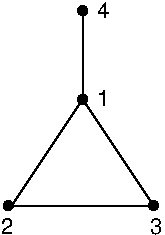
\includegraphics[scale=0.75]{./graph_example.pdf}
\end{minipage}
\hspace*{0.25in}
\begin{minipage}{0.4\textwidth}
%%\underline{\textsf{Local Functions:}}
\smallskip
\noindent
\begin{tabular}{|c|c|}\hline
\textbf{Node} & \textbf{Function} \\ \hline
1  &  OR \\ \hline
2  &  AND \\ \hline
3  &  NAND \\ \hline
4  &  NOR \\ \hline
\end{tabular}
\end{minipage}
\caption{\small{SyDS Example used to illustrate
the conversion predecessor problem to SAT.}}
\label{fig:syds_ex}
%%\rule{\textwidth}{0.01in}
\end{figure}
%%

\noindent
\textbf{Example:} Consider the SyDS example shown in Figure~\ref{fig:syds_ex}.
Suppose we want to find a predecessor of the configuration $(1, 0, 1, 0)$.
Using $x_1$, $x_2$, $x_3$ and $x_4$ to denote the Boolean variables corresponding
to the nodes 1, 2, 3 and 4, the Boolean formula to be satisfied when 
$(x_1, x_2, x_3, x_4)$ is a predecessor of $(1, 0, 1, 0)$ is:  

\medskip

\noindent
\hspace*{0.5in} $[1 ~\Leftrightarrow~ \mathrm{OR}(x_1, x_2, x_3, x_4)] ~\wedge~
[0 ~\Leftrightarrow~ \mathrm{AND}(x_1, x_2, x_3)] ~\wedge~ $\\
\hspace*{0.5in}
$[1 ~\Leftrightarrow~ \mathrm{NAND}(x_1, x_2, x_3)] ~\wedge~
[0 ~\Leftrightarrow~ \mathrm{NOR}(x_1, x_4)]$

\smallskip

\noindent
The above expression can be simplified to:

\begin{center}
$[\mathrm{OR}(x_1, x_2, x_3, x_4)] ~\wedge~
[\neg\,\mathrm{AND}(x_1, x_2, x_3)] ~\wedge~ 
[\mathrm{NAND}(x_1, x_2, x_3)] ~\wedge~
[\neg\,\mathrm{NOR}(x_1, x_4)]$
\end{center}

\noindent
By converting each subexpression above into its CNF equivalent, and
noticing that the term $[\mathrm{NAND}(x_1, x_2, x_3)]$ occurs twice
in the above expression, we get the following simplified
CNF formula:

\begin{center}
$(x_1 \vee  x_2 \vee  x_3 \vee  x_4)  ~\wedge~
(\overline{x_1} \vee \overline{x_2} \vee \overline{x_3}) ~\wedge~ 
(x_1 \vee x_4)$
\end{center}

%%\medskip

\noindent
\textbf{Note:}~ Simple constraints (such as requiring
the states of some nodes to be 0 and/or those of some nodes to be 1
in the predecessor) can be handled by inserting appropriate 
single literal clauses.
For example, if we require a predecessor in which node 1 is in state 0
and node 3 is in state 1, then we can add the single literal clauses
$\overline{x_1}$ and $x_3$ to the resulting CNF expression.
This illustrates an additional benefit of the SAT formulation.

\smallskip

\noindent
\textbf{Experimental Procedure and Results:}~ \textcolor{red}{(To be added.)}
            %%% Experimental results.

%\section{Conclusions and Future Research Directions}
%%\vspace*{-0.3in}
\section{Summary and Future Research Directions}
\label{sec:concl}
%%\vspace*{-.22in}

%%\textcolor{red}{(To be added.)} 
We investigated questions regarding the time evolution of
similar configurations.
We presented examples to show that SyDSs may exhibit
extreme behaviors in the evolution of configurations. 
In particular, our examples showed that in SyDSs, one may have
highly dissimilar configurations whose predecessors are similar.
Likewise, one may have very similar configurations whose predecessors
are highly dissimilar.
We also showed that the problem of computing similarity
measures of predecessors of given configurations is, in general,
computationally intractable.
We presented experimental results on similarity measures using
some restricted forms of underlying graphs and local functions.

There are several directions for future work.
For example, it is of interest to formally analyze the
behavior of restricted classes of SyDSs.
It will also be useful to identify restricted classes of SyDSs
for which similarity measures can be computed or approximated efficiently.
Finally, instead of considering one step predecessors, one may consider 
similarity issues for $t$-step predecessors for $t \geq 2$.

\smallskip

\noindent
\textbf{Acknowledgments:}~
This work has been partially supported by
DARPA Cooperative Agreement D17AC00003 (NGS2),
DTRA CNIMS (Contract HDTRA1-11-D-0016-0001),
NSF DIBBS Grant ACI-1443054,
NSF BIG DATA Grant IIS-1633028 and
NSF EAGER Grant CMMI-1745207.

%% \genprob{} for other uniform SyDSs,
%% \genprob{} with constraints to model fixed point
%% existence, etc. }

            %%% Conclusions and future work.

\iffalse
%%%%%
\noindent
\textbf{Acknowledgments:}~
We thank Professors Arun Phadke and late Jim Thorp for discussions related to problems studied in this paper.
This work has been partially supported by
DARPA Cooperative Agreement D17AC00003 (NGS2),
DTRA CNIMS (Contract HDTRA1-11-D-0016-0001),
NSF DIBBS Grant ACI-1443054, 
NSF BIG DATA Grant IIS-1633028 and
NSF EAGER Grant CMMI-1745207.
%The U.S. Government is authorized to reproduce and
%distribute reprints for Governmental purposes notwithstanding
%any copyright annotation thereon.
%%%%%%%
\fi

%%\vspace*{-.30in}

\bibliographystyle{splncs03}
%% \bibliographystyle{plain}
\bibliography{refs}

\end{document}
